\chapter{Gene Regulatory Networks: COMING SOON}
\label{ch_gene_reg_net}

Appendix \ref{ch-genomics-vocab}

\section{1 derivative (autoregulation) net}

\beq
\xymatrix{
f(\rvx)\ar[dr]|{1}
&&\rvx\ar[dl]|{-\alp}\ar[ll]
\\
&\Circle{\frac{d\rvx}{dt}}
}
\eeq
where $\alp >0$.

\beq
\frac{dx}{dt}=f(x)-\alp x
\eeq

\beq
f(x)=\left\{
\begin{array}{ll}
\beta\indi(x<K) 
&(f \text{ is lowpass})
\\
\beta\indi(x>K) 
&(f \text{ is highpass})
\end{array}
\right.
\eeq
where $\beta > 0$

\beq
x= x_0 e^{-\alp t} + f(x)
\left[ \frac{1-e^{-\alp t}}{\alp}\right]
\eeq

Three $x$ values $\{x_0, K, \frac{\beta}{\alp}\}$, and 
two $f$ values $\{ \text{lowpass, highpass}\}$

\begin{figure}[h!]
\centering
\includegraphics[width=3in]
{gene_reg_net/autoreg-approxs.png}
\caption{Approximations that we will use to understand the
gross behavior of the Autoreg net.
 }
\label{fig-autoreg-lowpass}
\end{figure}

\begin{figure}[h!]
\centering
\includegraphics[width=4in]
{gene_reg_net/autoreg-lowpass.png}
\caption{Autoreg net for lowpass $f$}
\label{fig-autoreg-lowpass}
\end{figure}

\begin{figure}[h!]
\centering
\includegraphics[width=4in]
{gene_reg_net/autoreg-highpass.png}
\caption{Autoreg net for highpass $f$}
\label{fig-autoreg-lowpass}
\label{fig-autoreg-highpass}
\end{figure}



\section{Single Input Module (SIM) net}

\section{Feedforward Loop (FFL) net}

\section{Bistable net}

\section{Biological clock net}